\documentclass[11pt,a4paper]{article}

% ─── PACKAGES ──────────────────────────────────────────────────────────────────
\usepackage[utf8]{inputenc}
\usepackage[T1]{fontenc}
\usepackage{amsmath,amssymb,amsthm}
\usepackage{mathtools}
\usepackage{geometry}
\usepackage{tikz}
\usepackage{pgfplots}
\usepackage{hyperref}
\usepackage{enumitem}
\usepackage{booktabs}
\usepackage{xcolor}
\usepackage{tcolorbox}
\usepackage{microtype}
\usepackage{titlesec}

\geometry{margin=1in}
\pgfplotsset{compat=1.18}

% ─── COLORS ────────────────────────────────────────────────────────────────────
\definecolor{accent}{HTML}{e8624a}
\definecolor{accentblue}{HTML}{5b8dee}
\definecolor{accentgreen}{HTML}{52c98d}
\definecolor{gold}{HTML}{d4a84b}
\definecolor{darkbg}{HTML}{0d0d0f}
\definecolor{mutedtext}{HTML}{7a7590}

% ─── THEOREM ENVIRONMENTS ──────────────────────────────────────────────────────
\newtheorem{theorem}{Theorem}
\newtheorem{proposition}[theorem]{Proposition}
\newtheorem{lemma}[theorem]{Lemma}
\newtheorem{corollary}[theorem]{Corollary}
\newtheorem{definition}[theorem]{Definition}
\theoremstyle{remark}
\newtheorem{remark}{Remark}

% ─── TCOLORBOX STYLES ─────────────────────────────────────────────────────────
\tcbuselibrary{skins,breakable}

% Legacy coloured environments render as plain remarks.
\newenvironment{keyresult}{\par\medskip\noindent\textit{Remark.}\ }{\par\medskip}
\newenvironment{geometricinsight}{\par\medskip\noindent\textit{Remark.}\ }{\par\medskip}
\newenvironment{casestudy}{\par\medskip\noindent\textit{Example.}\ }{\par\medskip}
\newenvironment{critique}{\par\medskip\noindent\textit{Remark.}\ }{\par\medskip}

% ─── HYPERREF SETUP ────────────────────────────────────────────────────────────
\hypersetup{
  colorlinks=true,
  linkcolor=accent,
  citecolor=accentblue,
  urlcolor=accentblue
}

% ─── TITLE ─────────────────────────────────────────────────────────────────────
\title{%
  \vspace{-1cm}
  {\Large\scshape On the Geometry of Difference in Representation Space}\\[0.6em]
  \textbf{Opposite $\neq$ Different:\\
  The Orthogonality Thesis}
}
\author{Taha Bouhsine\\[0.3em]{\normalsize\textit{azetta.ai}}}
\date{22 February 2026}

% ═══════════════════════════════════════════════════════════════════════════════
\begin{document}
\maketitle

% ─── ABSTRACT ──────────────────────────────────────────────────────────────────
\begin{abstract}
For unit vectors $\mathbf{u}, \mathbf{v} \in \mathbb{S}^{d-1}$ with $\cos\theta(\mathbf{u}, \mathbf{v}) = -1$, the relation $\mathbf{v} = -\mathbf{u}$ holds, so antiparallel vectors are linearly dependent and span a single line.
The maximally distinct configuration in the sense of linear independence is orthogonality, $\langle\mathbf{u}, \mathbf{v}\rangle = 0$, at which the span has dimension two and neither vector projects onto the other.
We collect the algebraic, information-theoretic, and packing-theoretic statements of this fact: the squared cosine $\cos^2\theta$ measures shared variance and is maximised at $\theta \in \{0, \pi\}$ and minimised at $\theta = \pi/2$; the regular simplex of $n$ unit vectors on $\mathbb{S}^{d-1}$ for $n \le d+1$ has pairwise cosine $-1/(n-1)$, which tends to zero as $n \to \infty$; the uniform distribution on $\mathbb{S}^{d-1}$ concentrates near orthogonality with $\mathrm{Var}[\cos\theta] = 1/d$.
We further show that cross-entropy, in the sense of the singularity $H(p,q) \to +\infty$ at $\mathrm{supp}(p) \cap \mathrm{supp}(q) = \varnothing$, registers disjoint support---the probabilistic analog of vector orthogonality---as an unbounded penalty, and that on the unit sphere the softmax classifier's equilibrium is the regular simplex.
A closing discussion (Section~\ref{sec:discussion}) examines what these statements imply for contrastive losses used in practice; that material is offered as motivation and consequence rather than as further theorems.
\end{abstract}

\tableofcontents
\vspace{1em}

% ═══════════════════════════════════════════════════════════════════════════════
\section{Introduction}
\label{sec:intro}
% ═══════════════════════════════════════════════════════════════════════════════

Cosine similarity is the standard measure of directional relationship between unit vectors on $\mathbb{S}^{d-1}$.
It ranges from $+1$ (parallel) through $0$ (orthogonal) to $-1$ (antiparallel).
A widely held convention treats the extremes of this range as a single ``difference'' axis, with $-1$ taken as the maximally distinct configuration.

Algebraically, this convention is incorrect.
Two unit vectors $\mathbf{u}, \mathbf{v} \in \mathbb{S}^{d-1}$ satisfying $\cos\theta(\mathbf{u}, \mathbf{v}) = -1$ also satisfy $\mathbf{v} = -\mathbf{u}$; they are linearly dependent and span a single line.
Genuine independence requires the span to have dimension at least two, and the cleanest realisation of that condition is orthogonality, $\langle\mathbf{u}, \mathbf{v}\rangle = 0$.
The aim of this paper is to collect the algebraic, information-theoretic, packing-theoretic, and probabilistic statements of this fact, and to discuss in a final section their implications for loss functions used in modern representation learning.

The paper is organised as follows.
Section~\ref{sec:geometry} establishes the algebra of linear dependence and independence on the sphere.
Section~\ref{sec:information} treats the information-theoretic counterpart in terms of $\cos^2\theta$.
Section~\ref{sec:concentration} records the concentration of $\cos\theta$ for uniform unit vectors on $\mathbb{S}^{d-1}$.
Section~\ref{sec:simplex} states the simplex packing result.
Section~\ref{sec:entropy} treats cross-entropy and the singularity at disjoint support.
Section~\ref{sec:discussion} is a closing discussion of contrastive losses in machine learning; that material is offered as motivation and consequence rather than as further theorems.


% ═══════════════════════════════════════════════════════════════════════════════
\section{The Geometry of Difference}
\label{sec:geometry}
% ═══════════════════════════════════════════════════════════════════════════════

We begin by formalising what ``different'' means in a vector space; the answer is not the answer most contrastive losses act on.

\begin{definition}[Linear dependence]
\label{def:lindep}
Two nonzero vectors $\mathbf{u}, \mathbf{v} \in \mathbb{R}^d$ are \emph{linearly dependent} if there exists $\alpha \in \mathbb{R} \setminus \{0\}$ such that $\mathbf{v} = \alpha \mathbf{u}$.
The span satisfies $\mathrm{span}(\mathbf{u}, \mathbf{v}) = \mathrm{span}(\mathbf{u})$, so $\dim \mathrm{span}(\mathbf{u}, \mathbf{v}) = 1$.
\end{definition}

\begin{theorem}[Antiparallel vectors are linearly dependent]
\label{thm:antiparallel}
Let $\mathbf{u}, \mathbf{v} \in \mathbb{S}^{d-1}$ with $\cos\theta(\mathbf{u}, \mathbf{v}) = -1$.
Then $\mathbf{v} = -\mathbf{u}$ and:
\begin{enumerate}[label=(\alph*)]
  \item $\mathrm{span}(\mathbf{u}, \mathbf{v}) = \mathrm{span}(\mathbf{u})$, so $\dim = 1$.
  \item The projection of $\mathbf{v}$ onto $\mathbf{u}$ is $\mathrm{proj}_\mathbf{u}(\mathbf{v}) = -\mathbf{u}$, with $|\mathrm{proj}_\mathbf{u}(\mathbf{v})| = \|\mathbf{u}\| = 1$.
  \item Knowing $\mathbf{u}$ determines $\mathbf{v}$ completely: $H(\mathbf{v} \mid \mathbf{u}) = 0$.
\end{enumerate}
\end{theorem}

\begin{proof}
Since $\mathbf{u}, \mathbf{v} \in \mathbb{S}^{d-1}$, we have $\|\mathbf{u}\| = \|\mathbf{v}\| = 1$.
The condition $\cos\theta = -1$ gives $\langle\mathbf{u}, \mathbf{v}\rangle = -1$.
Now consider $\|\mathbf{u} + \mathbf{v}\|^2 = \|\mathbf{u}\|^2 + 2\langle\mathbf{u}, \mathbf{v}\rangle + \|\mathbf{v}\|^2 = 1 - 2 + 1 = 0$.
Since $\|\mathbf{u} + \mathbf{v}\|^2 = 0$ implies $\mathbf{u} + \mathbf{v} = \mathbf{0}$, we have $\mathbf{v} = -\mathbf{u}$.
Parts (a)--(c) follow immediately: $\mathbf{v}$ is a scalar multiple of $\mathbf{u}$ with $\alpha = -1$.
\end{proof}

\begin{theorem}[Orthogonal vectors are maximally independent]
\label{thm:orthogonal}
Let $\mathbf{u}, \mathbf{v} \in \mathbb{S}^{d-1}$ with $\cos\theta(\mathbf{u}, \mathbf{v}) = 0$. Then:
\begin{enumerate}[label=(\alph*)]
  \item $\mathrm{span}(\mathbf{u}, \mathbf{v})$ has $\dim = 2$.
  \item $\mathrm{proj}_\mathbf{u}(\mathbf{v}) = \mathbf{0}$: $\mathbf{v}$ has zero component along $\mathbf{u}$.
  \item $\mathbf{v}$ cannot be reconstructed from $\mathbf{u}$ and vice versa.
\end{enumerate}
\end{theorem}

\begin{proof}
$\langle\mathbf{u}, \mathbf{v}\rangle = 0$ with $\mathbf{u}, \mathbf{v} \neq \mathbf{0}$ implies linear independence (standard result).
Hence $\dim\mathrm{span}(\mathbf{u}, \mathbf{v}) = 2$.
The projection $\mathrm{proj}_\mathbf{u}(\mathbf{v}) = \frac{\langle\mathbf{v}, \mathbf{u}\rangle}{\|\mathbf{u}\|^2}\mathbf{u} = 0 \cdot \mathbf{u} = \mathbf{0}$.
\end{proof}

\begin{keyresult}
The cosine scale has three landmarks, not two:
\begin{center}
\begin{tabular}{@{}lll@{}}
\toprule
$\cos\theta$ & Geometric status & Information content \\
\midrule
$+1$ & Parallel (identical direction) & Maximal redundancy \\
$-1$ & Antiparallel (opposite direction) & Maximal redundancy (sign-flipped) \\
$\phantom{-}0$ & Orthogonal (perpendicular) & Zero shared information \\
\bottomrule
\end{tabular}
\end{center}
The ``difference'' axis runs from $\pm 1$ (dependent) to $0$ (independent), not from $+1$ to $-1$.
\end{keyresult}

\begin{figure}[ht]
\centering
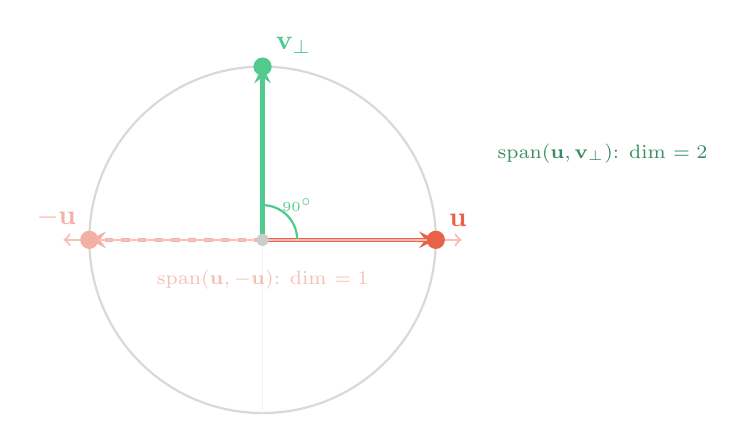
\begin{tikzpicture}[scale=2.2]
  % Unit circle
  \draw[thick, gray!30] (0,0) circle (1);

  % Quadrant guides
  \foreach \a in {0,90,180,270} {
    \draw[gray!10, very thin] (0,0) -- ({cos(\a)},{sin(\a)});
  }

  % Vector u
  \draw[accent, ultra thick, ->, >=stealth] (0,0) -- (1,0);
  \node[accent, font=\bfseries, anchor=south west] at (1.02,0.02) {$\mathbf{u}$};

  % Vector -u (antiparallel)
  \draw[accent!50, ultra thick, ->, >=stealth, dashed] (0,0) -- (-1,0);
  \node[accent!50, font=\bfseries, anchor=south east] at (-1.02,0.02) {$-\mathbf{u}$};

  % Vector v (orthogonal)
  \draw[accentgreen, ultra thick, ->, >=stealth] (0,0) -- (0,1);
  \node[accentgreen, font=\bfseries, anchor=south west] at (0.02,1.02) {$\mathbf{v}_\perp$};

  % Angle arc for orthogonal
  \draw[accentgreen, thick] (0.2,0) arc (0:90:0.2);
  \node[accentgreen, font=\tiny] at (0.2,0.2) {$90^\circ$};

  % Span annotation: antiparallel
  \draw[accent!40, thick, <->] (-1.15,0) -- (1.15,0);
  \node[accent!40, font=\scriptsize, anchor=north] at (0,-0.12) {$\mathrm{span}(\mathbf{u}, -\mathbf{u})$: dim $= 1$};

  % Span annotation: orthogonal
  \node[accentgreen!70!black, font=\scriptsize, anchor=west] at (1.3,0.5) {$\mathrm{span}(\mathbf{u}, \mathbf{v}_\perp)$: dim $= 2$};

  % Points
  \fill[accent] (1,0) circle (1.5pt);
  \fill[accent!50] (-1,0) circle (1.5pt);
  \fill[accentgreen] (0,1) circle (1.5pt);
  \fill[gray!40] (0,0) circle (1pt);
\end{tikzpicture}
\caption{Antiparallel vectors $\mathbf{u}$ and $-\mathbf{u}$ span a single line (dim $= 1$): they are linearly dependent.
The orthogonal vector $\mathbf{v}_\perp$ spans an independent direction (dim $= 2$): it carries genuinely new information.}
\label{fig:antiparallel-vs-orthogonal}
\end{figure}


% ═══════════════════════════════════════════════════════════════════════════════
\section{Softmax Contrastive Losses and Their Targets}
\label{sec:clip}
% ═══════════════════════════════════════════════════════════════════════════════

CLIP~\cite{radford2021clip} is the foundational model for modern vision--language systems, and its training objective is InfoNCE~\cite{oord2018infonce}: a softmax contrastive loss over a batch of $N$ image--text pairs.

\begin{definition}[InfoNCE / CLIP loss]
\label{def:infonce}
Given a batch of $N$ image-text pairs with embeddings $\{(\mathbf{z}^\text{img}_i, \mathbf{z}^\text{txt}_i)\}_{i=1}^N$, the InfoNCE loss for the image side is:
\begin{equation}
  \mathcal{L}_\text{CLIP} = -\frac{1}{N}\sum_{i=1}^N \log \frac{\exp\bigl(\mathrm{sim}(\mathbf{z}^\text{img}_i, \mathbf{z}^\text{txt}_i)/\tau\bigr)}{\sum_{k=1}^N \exp\bigl(\mathrm{sim}(\mathbf{z}^\text{img}_i, \mathbf{z}^\text{txt}_k)/\tau\bigr)},
  \label{eq:infonce}
\end{equation}
where $\mathrm{sim}(\mathbf{a}, \mathbf{b}) = \mathbf{a}^\top\mathbf{b} / (\|\mathbf{a}\|\|\mathbf{b}\|)$ is cosine similarity and $\tau > 0$ is a temperature.
\end{definition}

\begin{proposition}[InfoNCE implicitly targets antiparallel alignment]
\label{prop:infonce-target}
For a fixed anchor $\mathbf{z}^\text{img}_i$ and temperature $\tau > 0$, the InfoNCE gradient with respect to a negative embedding $\mathbf{z}^\text{txt}_k$ ($k \neq i$) pushes:
\begin{equation}
  \frac{\partial \mathcal{L}_\text{CLIP}}{\partial \mathrm{sim}(\mathbf{z}^\text{img}_i, \mathbf{z}^\text{txt}_k)} \propto \frac{\exp\bigl(\mathrm{sim}(\mathbf{z}^\text{img}_i, \mathbf{z}^\text{txt}_k)/\tau\bigr)}{\sum_{j=1}^N \exp\bigl(\mathrm{sim}(\mathbf{z}^\text{img}_i, \mathbf{z}^\text{txt}_j)/\tau\bigr)} > 0.
  \label{eq:infonce-grad}
\end{equation}
Since the gradient is strictly positive, the loss monotonically decreases as $\mathrm{sim}(\mathbf{z}^\text{img}_i, \mathbf{z}^\text{txt}_k)$ decreases.
The global minimum of each negative similarity is $-1$ (antiparallel), so InfoNCE drives negatives toward linear dependence with the anchor.
\end{proposition}

\begin{critique}
CLIP's InfoNCE loss wants ``a photo of a dog'' to be \emph{different} from ``a photo of a cat.''
But by driving their embeddings to $\cos = -1$, it makes the cat embedding a simple negation of the dog embedding.
The network doesn't learn that dogs and cats are different concepts; it learns they are opposite poles of the same axis.
One dimension consumed, zero new information.
\end{critique}

\subsection{Geometric Capacity Bound}

\begin{proposition}[Antiparallel capacity limit]
\label{prop:capacity}
In $\mathbb{R}^d$, the maximum number of mutually antiparallel unit vector pairs is $d$.
Each pair $(\mathbf{e}_i, -\mathbf{e}_i)$ consumes one basis direction.
\end{proposition}

\begin{proof}
Antiparallel pairs lie along one-dimensional subspaces.
Distinct one-dimensional subspaces of $\mathbb{R}^d$ correspond to points in the projective space $\mathbb{R}\mathbf{P}^{d-1}$.
For $n$ pairs to be mutually antiparallel, they must lie along $n$ distinct coordinate axes, and at most $d$ such orthogonal axes exist.
\end{proof}

\begin{corollary}
CLIP's 512-dimensional embedding space can represent at most 512 binary oppositions.
But ImageNet has 1,000 classes, and the real world has millions of concepts.
Any loss that targets $\cos = -1$ for all negative pairs faces a fundamental geometric impossibility.
\end{corollary}

\subsection{The Computational Catastrophe}

The geometric error compounds into a computational one.

\begin{proposition}[InfoNCE batch-size dependence]
\label{prop:batchsize}
The gradient signal for negative $k$ in InfoNCE is weighted by its softmax probability:
\begin{equation}
  w_k = \frac{\exp(\mathrm{sim}_k / \tau)}{\sum_{j} \exp(\mathrm{sim}_j / \tau)}.
  \label{eq:softmax-weight}
\end{equation}
In high dimensions, random unit vectors have $\mathrm{sim} \approx 0$ with variance $1/d$ (Theorem~\ref{thm:concentration}).
Consequently, most negatives contribute approximately equal, near-zero gradient, and the loss requires $N \gg 1$ to accumulate sufficient signal.
\end{proposition}

\begin{geometricinsight}
CLIP was trained with batch sizes of $N = 32{,}768$ image-text pairs.
Each batch requires computing an $N \times N$ similarity matrix ($\sim 4$ GB at float32).
This extreme cost is a direct consequence of the wrong geometric target:
\begin{itemize}
  \item The loss pushes negatives toward $\cos = -1$, but random embeddings are already near $\cos \approx 0$.
  \item Most of the batch contributes near-zero gradient---the loss has to see thousands of negatives to find the rare pairs near antiparallel alignment.
  \item The scaling law is brutal: doubling accuracy requires roughly quadrupling batch size.
\end{itemize}
The field spent years engineering distributed training, gradient caching, and memory-efficient attention---all to compensate for a geometric mistake in the loss function.
\end{geometricinsight}


% ═══════════════════════════════════════════════════════════════════════════════
\section{Sigmoid Pairwise Contrastive Losses}
\label{sec:siglip}
% ═══════════════════════════════════════════════════════════════════════════════

SigLIP~\cite{zhai2023siglip} replaces InfoNCE's softmax with a pairwise sigmoid.
The change is small in code and structural in geometry.

\begin{definition}[SigLIP loss]
\label{def:siglip}
Given image-text pairs with labels $y_{ij} = +1$ (matched) or $-1$ (mismatched):
\begin{equation}
  \mathcal{L}_\text{SigLIP} = \sum_{i,j} \log\bigl(1 + \exp\bigl(-y_{ij}\bigl(\mathrm{sim}(\mathbf{z}_i, \mathbf{z}_j)/\tau - b\bigr)\bigr)\bigr),
  \label{eq:siglip}
\end{equation}
where $b$ is a learnable bias parameter.
\end{definition}

\begin{proposition}[Sigmoid equilibrium at orthogonality]
\label{prop:siglip-equilibrium}
For a mismatched pair ($y_{ij} = -1$), the SigLIP gradient with respect to similarity is:
\begin{equation}
  \frac{\partial \mathcal{L}}{\partial \mathrm{sim}_{ij}} = \frac{1}{\tau} \cdot \sigma\bigl(\mathrm{sim}_{ij}/\tau - b\bigr),
  \label{eq:siglip-grad}
\end{equation}
where $\sigma$ is the logistic sigmoid.
This gradient vanishes as $\mathrm{sim}_{ij} \to -\infty$, but in practice the sigmoid saturates once $\mathrm{sim}_{ij} < b$ by a few multiples of $\tau$.
Unlike InfoNCE, SigLIP does \emph{not} push similarity toward $-1$---it only requires $\mathrm{sim}_{ij} < b$.
\end{proposition}

\begin{theorem}[Concentration of measure on $\mathbb{S}^{d-1}$]
\label{thm:concentration}
For two independent uniform random vectors $\mathbf{x}, \mathbf{y} \sim \mathrm{Uniform}(\mathbb{S}^{d-1})$:
\begin{equation}
  \mathbb{E}[\cos\theta(\mathbf{x}, \mathbf{y})] = 0, \qquad \mathrm{Var}[\cos\theta(\mathbf{x}, \mathbf{y})] = \frac{1}{d}.
  \label{eq:concentration}
\end{equation}
For $d = 512$ (CLIP's embedding dimension), $\mathrm{Std}[\cos\theta] \approx 0.044$.
Almost all pairs of random unit vectors are nearly orthogonal.
\end{theorem}

\begin{proof}
Let $\mathbf{y} = (Y_1, \dots, Y_d)^\top$ be uniform on $\mathbb{S}^{d-1}$.
Without loss of generality, fix $\mathbf{x} = \mathbf{e}_1$.
Then $\cos\theta = Y_1$.
The marginal distribution of $Y_1$ for the uniform distribution on $\mathbb{S}^{d-1}$ has $\mathbb{E}[Y_1] = 0$ (by symmetry) and $\mathrm{Var}[Y_1] = \mathbb{E}[Y_1^2] = \frac{1}{d}$ (since $\sum_i Y_i^2 = 1$ and all components have equal variance).
\end{proof}

\begin{keyresult}
SigLIP's sigmoid loss aligns with the natural geometry of high-dimensional spheres:
\begin{itemize}
  \item Random embeddings are already near $\cos \approx 0$ (orthogonal).
  \item The sigmoid only needs mismatched similarities below the bias $b$---it doesn't fight the geometry by pushing toward $-1$.
  \item The pairwise structure eliminates the $N \times N$ softmax competition, enabling smaller batch sizes.
\end{itemize}
Result: better zero-shot accuracy with less compute~\cite{zhai2023siglip}.
Not because of better engineering, but because the geometry is right.
\end{keyresult}


% ═══════════════════════════════════════════════════════════════════════════════
\section{Cross-Entropy at Disjoint Support}
\label{sec:entropy}
% ═══════════════════════════════════════════════════════════════════════════════

Cross-entropy is the standard classification loss.
The geometry it has always been driving toward is orthogonality, not opposition---a fact obscured by the way the loss is usually described, but visible immediately in its singularity structure.

\begin{definition}[Cross-entropy]
For discrete distributions $p$ and $q$ over alphabet $\mathcal{X}$:
\begin{equation}
  H(p, q) = -\sum_{x \in \mathcal{X}} p(x) \log q(x).
  \label{eq:cross-entropy}
\end{equation}
\end{definition}

\begin{theorem}[Singularity at disjoint support]
\label{thm:singularity}
If $\mathrm{supp}(p) \cap \mathrm{supp}(q) = \varnothing$, then $H(p, q) = +\infty$.
\end{theorem}

\begin{proof}
If the supports are disjoint, then for every $x$ with $p(x) > 0$ we have $q(x) = 0$, so $\log q(x) = -\infty$.
Since $p(x) > 0$ for at least one such $x$:
\[
  H(p,q) = -\sum_{x} p(x) \log q(x) \geq -p(x_0) \log q(x_0) = -p(x_0) \cdot (-\infty) = +\infty.
\]
\end{proof}

\begin{geometricinsight}
Disjoint support is the probabilistic analog of orthogonality.
Two distributions whose supports don't intersect are like two vectors with zero dot product: they share no information, they occupy independent regions of the sample space.
The singularity $H(p,q) \to +\infty$ is cross-entropy's way of encoding complete orthogonality.
\end{geometricinsight}

\subsection{Why Classifiers Learn Orthogonal Representations}

\begin{proposition}[Softmax drives orthogonal weight vectors]
\label{prop:softmax-orthogonal}
In a softmax classifier with logits $z_k = \mathbf{w}_k^\top \mathbf{h}$ and cross-entropy loss, the gradient with respect to the wrong-class logit $z_k$ ($k \neq y$) is:
\begin{equation}
  \frac{\partial \mathcal{L}}{\partial z_k} = \hat{p}(k \mid \mathbf{h}) = \frac{\exp(z_k)}{\sum_j \exp(z_j)} > 0.
  \label{eq:ce-gradient}
\end{equation}
This gradient pushes $z_k = \mathbf{w}_k^\top \mathbf{h}$ toward $-\infty$.
On the unit sphere ($\|\mathbf{w}_k\| = \|\mathbf{h}\| = 1$), the loss has competing pressures: it wants $\mathbf{w}_y$ parallel to $\mathbf{h}$ (to maximise $z_y$) and each $\mathbf{w}_k$ with $k \neq y$ antiparallel to $\mathbf{h}$ (to minimise $z_k$).
With $n$ classes sharing the same $\mathbf{h}$, the antiparallel target cannot be reached simultaneously by all $\mathbf{w}_k$, so the equilibrium is determined by the configuration that minimises the wrong-class logits subject to mutual diversity of the $\mathbf{w}_k$.
That configuration is the regular simplex (Theorem~\ref{thm:simplex}): $\langle \mathbf{w}_k, \mathbf{h}\rangle = -1/(n-1)$ for all $k \neq y$, which tends to $0$ as $n$ grows.
The equilibrium is therefore \emph{approximately} orthogonal for any non-trivial multi-class setting and \emph{exactly} orthogonal in the limit $n \to \infty$; the binary case $n = 2$ is the only regime in which the equilibrium is genuinely antiparallel.
\end{proposition}

\begin{casestudy}
This explains why plain cross-entropy classifiers produce well-separated representations even without any contrastive mechanism:
\begin{itemize}
  \item The loss's singularity structure is geometrically informed by orthogonality.
  \item SigLIP's sigmoid loss shares this singularity structure (binary cross-entropy per pair), which is why it naturally drives mismatched pairs to orthogonality.
  \item CLIP's softmax InfoNCE does \emph{not} share this structure---its softmax competition pushes beyond orthogonality toward opposition.
\end{itemize}
\end{casestudy}


% ═══════════════════════════════════════════════════════════════════════════════
\section{Optimal Packing on the Sphere}
\label{sec:simplex}
% ═══════════════════════════════════════════════════════════════════════════════

What is the optimal arrangement of $n$ class representations on $\mathbb{S}^{d-1}$ when $n \leq d + 1$?

\begin{theorem}[Regular simplex packing]
\label{thm:simplex}
The arrangement of $n$ unit vectors on $\mathbb{S}^{d-1}$ that maximizes the minimum pairwise angle (the Tammes problem for $n \leq d+1$) is the regular simplex, where all pairwise cosine similarities are equal:
\begin{equation}
  \cos\theta_{ij} = -\frac{1}{n-1} \quad \text{for all } i \neq j.
  \label{eq:simplex}
\end{equation}
\end{theorem}

\begin{proof}[Proof sketch]
The $n$ vertices of a regular simplex centered at the origin in $\mathbb{R}^n$ satisfy $\sum_{i=1}^n \mathbf{v}_i = \mathbf{0}$ and $\|\mathbf{v}_i\| = c$ for all $i$.
Computing:
\[
  \mathbf{0} = \Bigl\|\sum_i \mathbf{v}_i\Bigr\|^2 = \sum_i \|\mathbf{v}_i\|^2 + 2\sum_{i<j} \langle\mathbf{v}_i, \mathbf{v}_j\rangle = nc^2 + 2\binom{n}{2}\langle\mathbf{v}_i, \mathbf{v}_j\rangle,
\]
where the last equality uses equi-angularity.
Solving: $\cos\theta = \langle\mathbf{v}_i, \mathbf{v}_j\rangle/c^2 = -\frac{1}{n-1}$.
For $n \leq d+1$, this configuration embeds in $\mathbb{S}^{d-1}$.
\end{proof}

\begin{corollary}[Simplex approaches orthogonality]
\label{cor:simplex-limit}
As the number of classes grows:
\[
  \lim_{n \to \infty} \cos\theta_\text{simplex} = \lim_{n \to \infty} \left(-\frac{1}{n-1}\right) = 0.
\]
The optimal packing converges to orthogonality, not opposition.
\end{corollary}

\begin{figure}[ht]
\centering
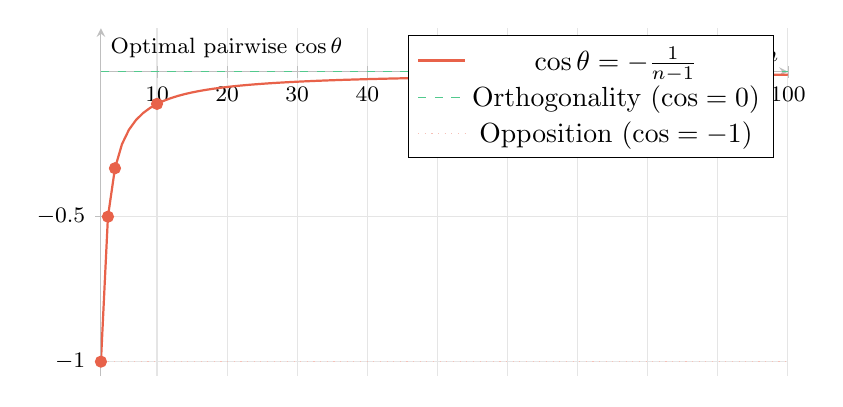
\begin{tikzpicture}
  \begin{axis}[
    width=0.85\textwidth,
    height=6cm,
    xlabel={Number of classes $n$},
    ylabel={Optimal pairwise $\cos\theta$},
    xmin=2, xmax=100,
    ymin=-1.05, ymax=0.15,
    ytick={-1, -0.5, 0},
    grid=major,
    grid style={gray!20},
    axis lines=middle,
    axis line style={gray!50},
    tick style={gray!50},
    every axis label/.style={font=\footnotesize},
    every tick label/.style={font=\footnotesize},
  ]
    % Simplex curve
    \addplot[accent, thick, domain=2:100, samples=99] {-1/(x-1)};
    \addlegendentry{$\cos\theta = -\frac{1}{n-1}$}

    % Asymptote at 0
    \addplot[accentgreen, dashed, domain=2:100] {0};
    \addlegendentry{Orthogonality ($\cos = 0$)}

    % Opposition line
    \addplot[accent!40, dotted, domain=2:100] {-1};
    \addlegendentry{Opposition ($\cos = -1$)}

    % Key points
    \addplot[only marks, mark=*, mark size=2pt, accent] coordinates {(2,-1) (3,-0.5) (4,-0.333) (10,-0.111) (50,-0.0204)};

  \end{axis}
\end{tikzpicture}
\caption{The optimal inter-class cosine similarity for $n$ classes on the simplex.
For $n = 2$ (binary), the optimal angle is $180^\circ$ ($\cos = -1$)---opposition works.
But for $n \geq 3$, the optimal configuration rapidly approaches orthogonality.
By $n = 10$, $\cos\theta \approx -0.11$; by $n = 50$, $\cos\theta \approx -0.02$.
Contrastive losses that target $\cos = -1$ for all negatives are fighting the geometry.}
\label{fig:simplex}
\end{figure}

\begin{remark}
The simplex result explains a striking empirical observation: for binary classification ($n = 2$), the optimal arrangement \emph{is} antiparallel ($\cos = -1$), and standard contrastive losses work well.
The confusion arises from over-generalizing the binary case to multi-class settings, where opposition becomes increasingly wrong.
\end{remark}


% ═══════════════════════════════════════════════════════════════════════════════
\section{Directional Mutual Information}
\label{sec:information}
% ═══════════════════════════════════════════════════════════════════════════════

We can also frame the distinction in information-theoretic terms.

\begin{definition}[Directional mutual information]
For unit vectors $\mathbf{u}, \mathbf{v} \in \mathbb{S}^{d-1}$, define the directional mutual information as:
\begin{equation}
  I_\text{dir}(\mathbf{u}; \mathbf{v}) = 1 - \frac{\|\mathbf{v} - \mathrm{proj}_\mathbf{u}(\mathbf{v})\|^2}{\|\mathbf{v}\|^2} = \cos^2\theta(\mathbf{u}, \mathbf{v}).
  \label{eq:dir-mi}
\end{equation}
This measures the fraction of $\mathbf{v}$'s variance explained by $\mathbf{u}$.
\end{definition}

\begin{proposition}[Antiparallel maximizes shared information]
\label{prop:mi-antiparallel}
\begin{align}
  \cos\theta = -1 &\;\Longrightarrow\; I_\text{dir} = \cos^2\theta = 1 & \text{(maximal redundancy)}, \\
  \cos\theta = \phantom{-}0 &\;\Longrightarrow\; I_\text{dir} = \cos^2\theta = 0 & \text{(zero shared info)}, \\
  \cos\theta = +1 &\;\Longrightarrow\; I_\text{dir} = \cos^2\theta = 1 & \text{(maximal redundancy)}.
\end{align}
Both parallel \emph{and} antiparallel vectors share all information.
Only orthogonal vectors share none.
\end{proposition}

\begin{keyresult}
The true ``difference'' metric is $\cos^2\theta$, not $\cos\theta$.
It is minimized at orthogonality, not at opposition:
\begin{equation}
  \boxed{\,\text{max difference} \;\Longleftrightarrow\; \cos^2\theta = 0 \;\Longleftrightarrow\; \cos\theta = 0 \;\Longleftrightarrow\; \mathbf{u} \perp \mathbf{v}\,}
  \label{eq:thesis}
\end{equation}
\end{keyresult}


\begin{figure}[ht]
\centering
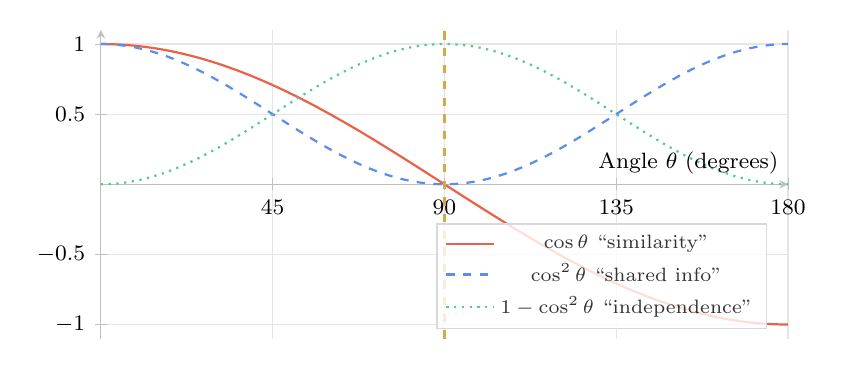
\begin{tikzpicture}
  \begin{axis}[
    width=0.85\textwidth,
    height=5.5cm,
    xlabel={Angle $\theta$ (degrees)},
    ylabel={},
    xmin=0, xmax=180,
    ymin=-1.1, ymax=1.1,
    xtick={0,45,90,135,180},
    ytick={-1, -0.5, 0, 0.5, 1},
    grid=major,
    grid style={gray!20},
    axis lines=middle,
    axis line style={gray!50},
    tick style={gray!50},
    every axis label/.style={font=\footnotesize},
    every tick label/.style={font=\footnotesize},
    legend pos=south east,
    legend style={font=\scriptsize, fill=white, fill opacity=0.8, draw=gray!30},
  ]
    % cos theta
    \addplot[accent, thick, domain=0:180, samples=200] {cos(x)};
    \addlegendentry{$\cos\theta$ ``similarity''}

    % cos^2 theta
    \addplot[accentblue, thick, dashed, domain=0:180, samples=200] {cos(x)^2};
    \addlegendentry{$\cos^2\theta$ ``shared info''}

    % 1 - cos^2 theta (independence)
    \addplot[accentgreen, thick, dotted, domain=0:180, samples=200] {1 - cos(x)^2};
    \addlegendentry{$1 - \cos^2\theta$ ``independence''}

    % Vertical line at 90
    \addplot[gold, thick, dashed] coordinates {(90,-1.1) (90,1.1)};

  \end{axis}
\end{tikzpicture}
\caption{The similarity $\cos\theta$ (red) reaches its minimum at $\theta = 180^\circ$, but the shared information $\cos^2\theta$ (blue dashed) is \emph{maximized} at both $0^\circ$ and $180^\circ$.
True independence $1 - \cos^2\theta$ (green dotted) peaks at $\theta = 90^\circ$: \textbf{orthogonality}.
The gold line marks the point of maximum difference.}
\label{fig:info-curves}
\end{figure}


% ═══════════════════════════════════════════════════════════════════════════════
\section{Discussion}
\label{sec:discussion}
% ═══════════════════════════════════════════════════════════════════════════════

\begin{table}[ht]
\centering
\caption{Comparison of loss functions and their geometric targets.}
\label{tab:comparison}
\begin{tabular}{@{}lcccc@{}}
\toprule
\textbf{Method} & \textbf{Loss type} & \textbf{Negative target} & \textbf{Batch req.} & \textbf{Geometry} \\
\midrule
SimCLR~\cite{chen2020simclr} & Softmax InfoNCE & $\cos \to -1$ & $N \geq 4096$ & Opposition \\
CLIP~\cite{radford2021clip} & Softmax InfoNCE & $\cos \to -1$ & $N = 32768$ & Opposition \\
SigLIP~\cite{zhai2023siglip} & Sigmoid pairwise & $\cos < b$ & $N \geq 1024$ & Orthogonality \\
Cross-entropy & Softmax CE & $z_k \to 0$ & N/A & Orthogonality \\
SupCon~\cite{khosla2020supcon} & Supervised InfoNCE & $\cos \to -1$ & $N \geq 2048$ & Opposition \\
\bottomrule
\end{tabular}
\end{table}

\begin{keyresult}
The methods that target orthogonality (SigLIP, cross-entropy) share two properties:
\begin{enumerate}
  \item They align with the natural concentration of measure on $\mathbb{S}^{d-1}$.
  \item They achieve comparable or better accuracy with less compute.
\end{enumerate}
The methods that target opposition (SimCLR, CLIP, SupCon) require enormous batch sizes to overcome the geometric tension between their objective and the high-dimensional geometry of the sphere.
\end{keyresult}


The point of the present paper is that the algebraic distinction between dependence and independence (Section~\ref{sec:geometry}), the information-theoretic counterpart (Section~\ref{sec:information}), the packing geometry of the regular simplex on $\mathbb{S}^{d-1}$ (Section~\ref{sec:simplex}), and the disjoint-support singularity of cross-entropy (Section~\ref{sec:entropy}) all identify the same configuration: orthogonality is the maximally distinct configuration in every formulation under consideration, and opposition is its redundant counterpart.
This identification is mathematically straightforward; the consequences for losses used in practice are interpretive, and we have tried to mark the boundary throughout.


% ═══════════════════════════════════════════════════════════════════════════════
% REFERENCES
% ═══════════════════════════════════════════════════════════════════════════════
\begin{thebibliography}{10}

\bibitem{radford2021clip}
A.~Radford, J.~W. Kim, C.~Hallacy, A.~Ramesh, G.~Goh, S.~Agarwal, G.~Sastry, A.~Askell, P.~Mishkin, J.~Clark, G.~Krueger, and I.~Sutskever.
\newblock Learning transferable visual models from natural language supervision.
\newblock In \emph{Proceedings of ICML}, 2021.
\newblock \url{https://arxiv.org/abs/2103.00020}

\bibitem{zhai2023siglip}
X.~Zhai, B.~Mustafa, A.~Kolesnikov, and L.~Beyer.
\newblock Sigmoid loss for language image pre-training.
\newblock In \emph{Proceedings of ICCV}, 2023.
\newblock \url{https://arxiv.org/abs/2303.15343}

\bibitem{chen2020simclr}
T.~Chen, S.~Kornblith, M.~Norouzi, and G.~Hinton.
\newblock A simple framework for contrastive learning of visual representations.
\newblock In \emph{Proceedings of ICML}, 2020.
\newblock \url{https://arxiv.org/abs/2002.05709}

\bibitem{oord2018infonce}
A.~van~den~Oord, Y.~Li, and O.~Vinyals.
\newblock Representation learning with contrastive predictive coding.
\newblock \emph{arXiv preprint arXiv:1807.03748}, 2018.
\newblock \url{https://arxiv.org/abs/1807.03748}

\bibitem{khosla2020supcon}
P.~Khosla, P.~Teterwak, C.~Wang, A.~Sarna, Y.~Tian, P.~Isola, A.~Maschinot, C.~Liu, and D.~Krishnan.
\newblock Supervised contrastive learning.
\newblock In \emph{Advances in NeurIPS}, 2020.
\newblock \url{https://arxiv.org/abs/2004.11362}

\bibitem{steck2024}
H.~Steck, C.~Ekanadham, and N.~Kallus.
\newblock Is cosine-similarity of learned representations all you need?
\newblock \emph{arXiv preprint arXiv:2403.05440}, 2024.
\newblock \url{https://arxiv.org/abs/2403.05440}

\bibitem{wang2020hypersphere}
T.~Wang and P.~Isola.
\newblock Understanding contrastive representation learning through alignment and uniformity on the hypersphere.
\newblock In \emph{Proceedings of ICML}, 2020.
\newblock \url{https://arxiv.org/abs/2005.10242}

\end{thebibliography}

\end{document}
